\section{Diseño}

En esta etapa de la metodología ágil, se debe elaborar un diseño que responda a las dificultades que los adultos mayores puedan experimentar probando juegos digitales. Encontrar el punto medio entre entretenimiento y aprendizaje, hacer una correcta integración de los elementos visuales y garantizar la legibilidad son algunos de los aspectos que se tratarán en este apartado.

\subsection{Diseño de la arquitectura}

La arquitectura completa de la skill se construirá sobre varias herramientas de \textit{Amazon Web Services} (AWS) que serán explicadas con mayor detalle en la sección 6. Estas se encuentran englobadas en \textit{AWS Serverless Platform}, una plataforma que permite la creación de skills sin necesidad de disponer de un servidor propio. 

Las tecnologías avanzadas de AWS más relevantes en el desarrollo de skills son: AWS Lambda, Amazon DynamoDB y Amazon S3. Estas se integran de la forma descrita en la \autoref{fig:arquitectura-skill}.

\begin{figure}[H]
	\centering
	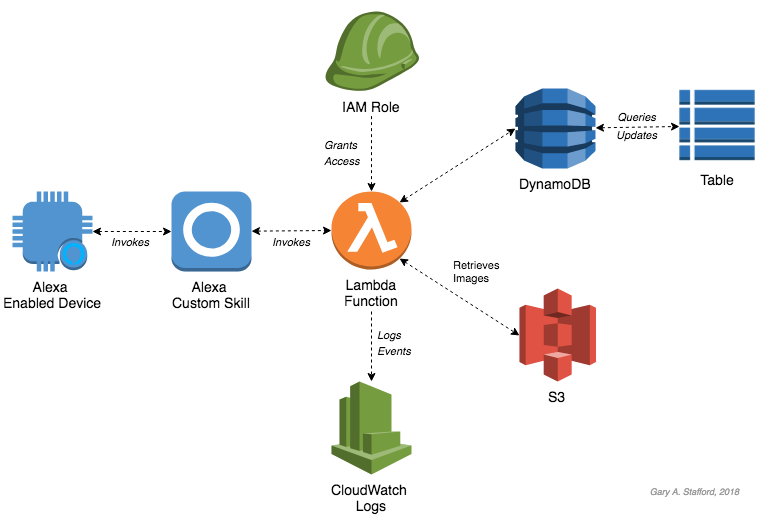
\includegraphics[width=0.98\textwidth]{imgs/arquitectura-skill.png}
	\caption{Arquitectura de una skill de Alexa con las tecnologías AWS \parencite{arquitecturaSkill}}
	\label{fig:arquitectura-skill}
\end{figure}

\newpage

El proceso de creación de la habilidad para Alexa implica varios pasos clave \parencite{arquitecturaSkill}:
\begin{enumerate}
	\item Definir el modelo de interacción por voz; es decir, cómo los usuarios pueden invocar la skill con diversas intenciones mediante comandos de voz.
	\item Diseñar la interfaz, solo en caso de que se vaya a desplegar en dispositivos con pantallas, para mejorar la experiencia de usuario al mostrar información visual complementaria al audio.
	\item Configurar las tablas en DynamoDB: para el almacenamiento persistente de información, usando una base de datos.
	\item Crear un bucket en S3 donde se alojarán las imágenes y vídeos requeridos para el paso 2.
	\item Programar la skill de Alexa, con funciones que permitan gestionar el flujo de conversación entre los usuarios y Alexa.
	\item Escribir la función Lambda, responsable de procesar las entradas del usuario y devolver las respuestas adecuadas, que peuden incluir datos almacenados en DynamoDB y en S3.
	\item Modificar el rol IAM predeterminado para que la función Lambda actualice la información de la base de datos según sea necesario.
	\item Desplegar y probar la skill para asegurarse de que funciona según lo esperado.
\end{enumerate}

Adicionalmente, para gestionar los elementos visuales que serán mostrados en la pantalla del dispositivo, se tiene la siguiente arquitectura para el Lenguaje de Presentación de Alexa, comúnmente conocido como APL (\autoref{fig:arquitectura-apl}).

\begin{figure}[H]
	\centering
	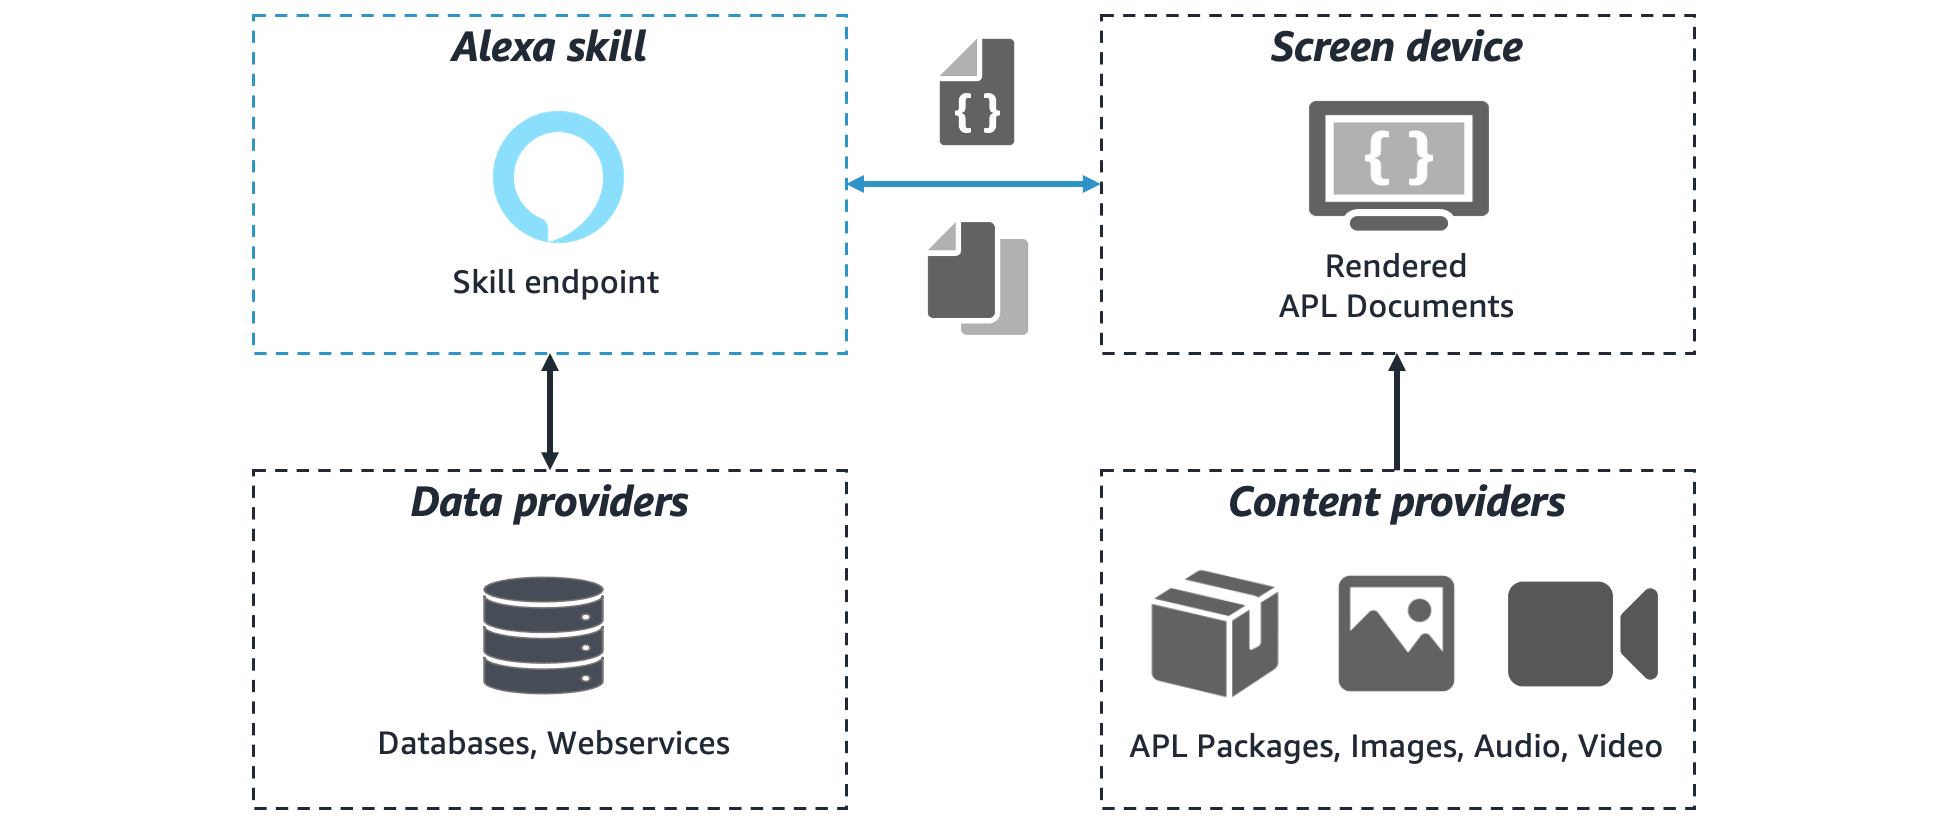
\includegraphics[width=0.98\textwidth]{imgs/arquitectura-apl.png}
	\caption{Arquitectura de una APL con los cuatro actores principales (\href{https://developer.amazon.com/en-US/docs/alexa/alexa-presentation-language/apl-bp-understand-apl-architecture.html}{Alexa Developer Docs})}
\label{fig:arquitectura-apl}
\end{figure}

Los dos agentes esenciales son:
\begin{itemize}
	\item \textbf{La propia skill}: es la que inicia el proceso al enviar primero la plantilla del documento APL al dispositivo.
	\item \textbf{Los dispositivos con pantalla}: algunos dispositivos Alexa, como el Echo Show, son compatibles con este lenguaje de presentación y se encargan de mostrar por pantalla la plantilla APL. 
\end{itemize}

Los anteriores pueden ser complementados por agentes opcionales como: 
\begin{itemize}
	\item \textbf{Los proveedores de datos}: normalmente bases de datos como DynamoDB, almacenan de forma externa a la skill información relevante que puede ser consultada y/o modificada.
	\item \textbf{Los proveedores de contenido}: como Amazon S3, que incluyen archivos multimedia externos, que se almacenan públicamente en la red y son referenciados desde la skill mediante URLs. 
\end{itemize}

\subsection{GDD: Documento de Diseño del Juego}

Como bien se menciona en el libro \textit{Game design workshop: a playcentric approach to creating innovative games} \parencite{fullerton2008game}, el Game Design Document (GDD) es un documento que integra todos los aspectos relevantes de un videojuego, desde la mecánica y la narrativa hasta los elementos visuales y de audio. 

Es útil porque sirve como roadmap (plan estratégico para alcanzar unos determinados objetivos a largo plazo) para todo el proceso de desarrollo, así como una guía para coordinar las tareas de los miembros del equipo a lo largo del camino hacia alcanzar dichos objetivos.

Se ha hecho una adaptación a una plantilla de uso gratuito para elaborar el documento de diseño del juego mostrado en la \autoref{fig:GDD-imagen}. 

\begin{figure}[H]
	\centering
	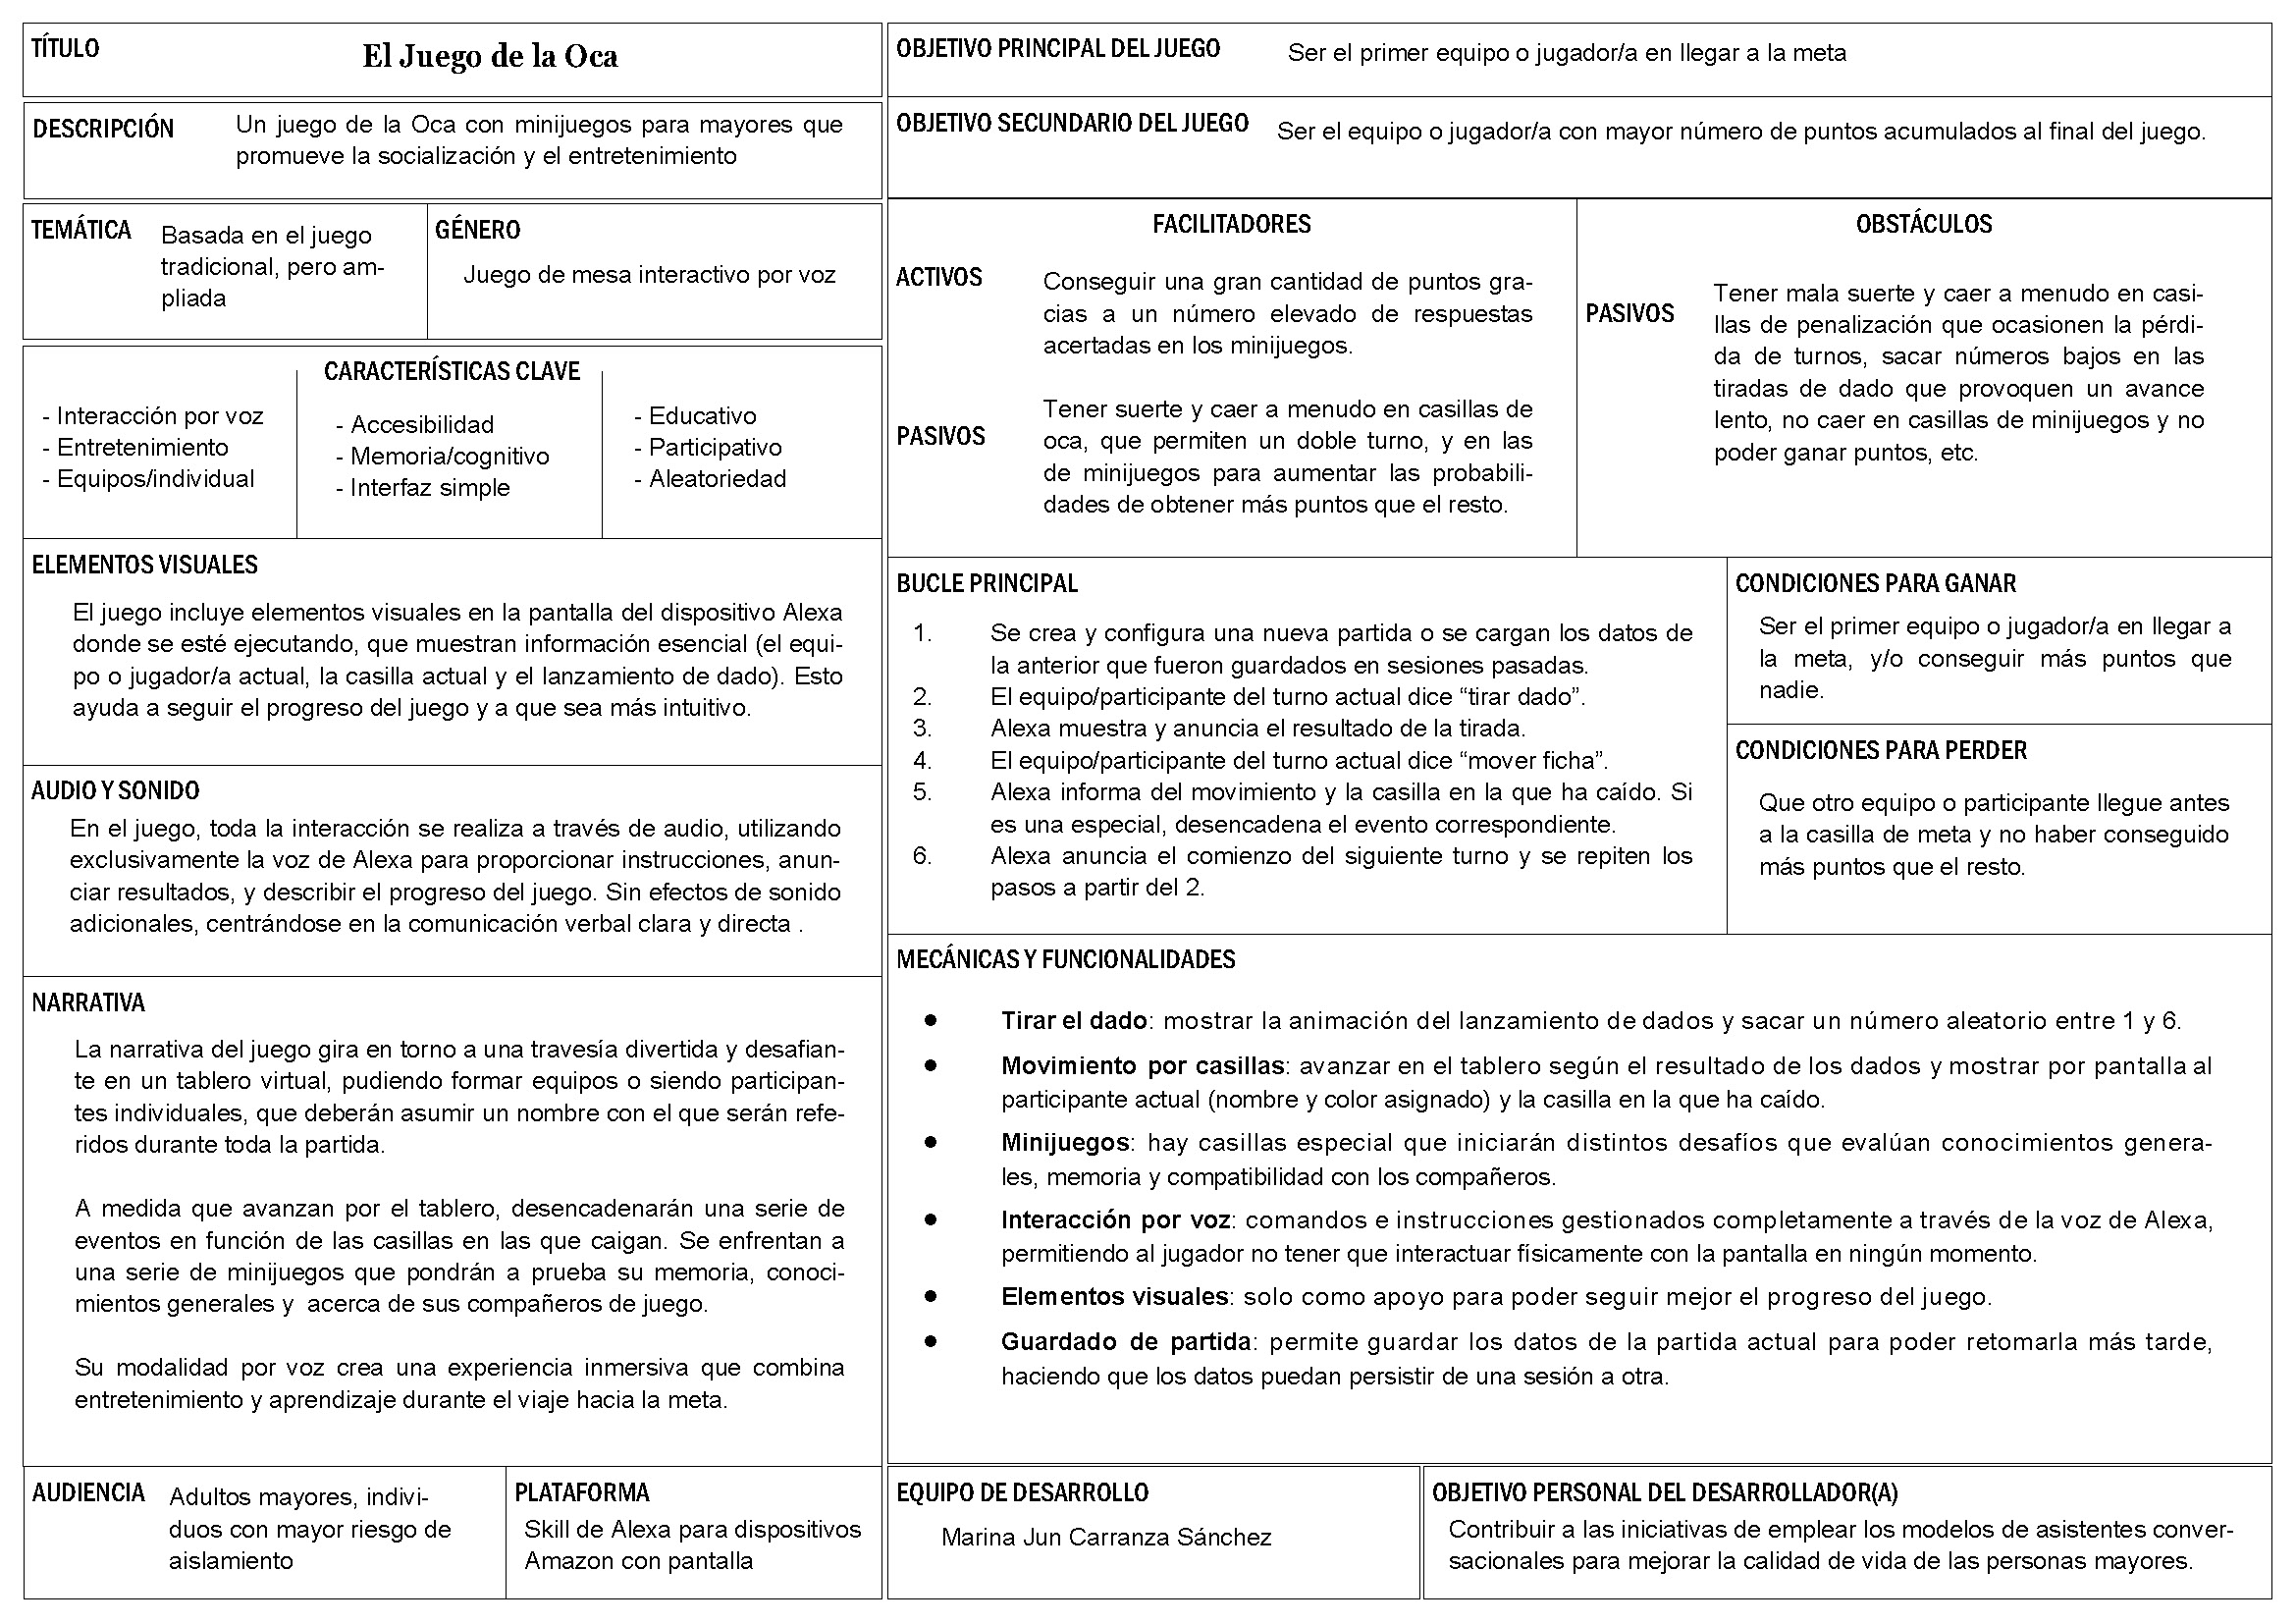
\includegraphics[width=1\textwidth]{imgs/GDD-imagen.jpg}
	\caption{Game Design Document}
	\label{fig:GDD-imagen}
\end{figure}

\subsection{Modelo conceptual del juego de la oca}

Aunque en una skill de Alexa los modelos conceptuales no se ajustan de la misma forma que lo harían en un sistema orientado a objetos tradicional, sí se puede plantear un diagrama de conceptos que encapsule las clases del juego de la oca y cómo se relacionan entre sí.

Se ha ilustrado el diagrama conceptual de forma aislada a la estructura particular de la skill en la \autoref{fig:DConcep-1}:

\vline
\begin{figure}[H]
	\centering
	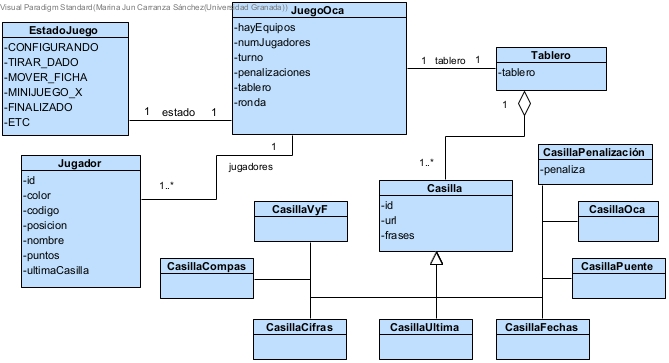
\includegraphics[width=1\textwidth]{imgs/DConcep.jpg}
	\caption{Diagrama conceptual del juego de la oca (\href{https://www.visual-paradigm.com/}{\textit{Visual Paradigm}})}
	\label{fig:DConcep-1}
\end{figure}

Dicho diagrama de conceptos describe la estructura y relaciones principales del juego de la oca. 

\textit{JuegoOca} es la clase central que gestiona el juego, incluyendo aspectos como el tipo de participantes, el número de ellos, el turno actual... Además, cada instancia del juego de la oca tiene asociados:
\begin{itemize}
	\item Un estado de juego, definido por el enumerado \textit{EstadoJuego}, que indica el punto en el que se encuentra una partida.
	\item Un tablero, compuesto por varias instancias de la clase \textit{Casilla}. Estas a su vez pueden ser de distintos tipos, en función del efecto que provoquen cuando alguien cae en ellas (penalizaciones, ocas, puentes, etc).
	\item Una o más instancias de la clase \textit{Jugador}, que representa a cada participante del juego con atributos como su id, nombre, color, puntos...
\end{itemize}

El diseño de este diagrama organiza de manera clara los elementos y su interacción en el juego de la oca, facilitando en gran medida su futura implementación.

\newpage 

\subsection{Diseño de la interfaz de usuario}

Aunque no se vaya a mostrar entero en la pantalla del dispositivo, se ha realizado un diseño con Adobe Photoshop del tablero que utilizará la skill (\autoref{fig:tablero-oca}), lo que ha ayudado a visualizarlo y facilitar su implementación más adelante.

\begin{figure}[H]
	\centering
	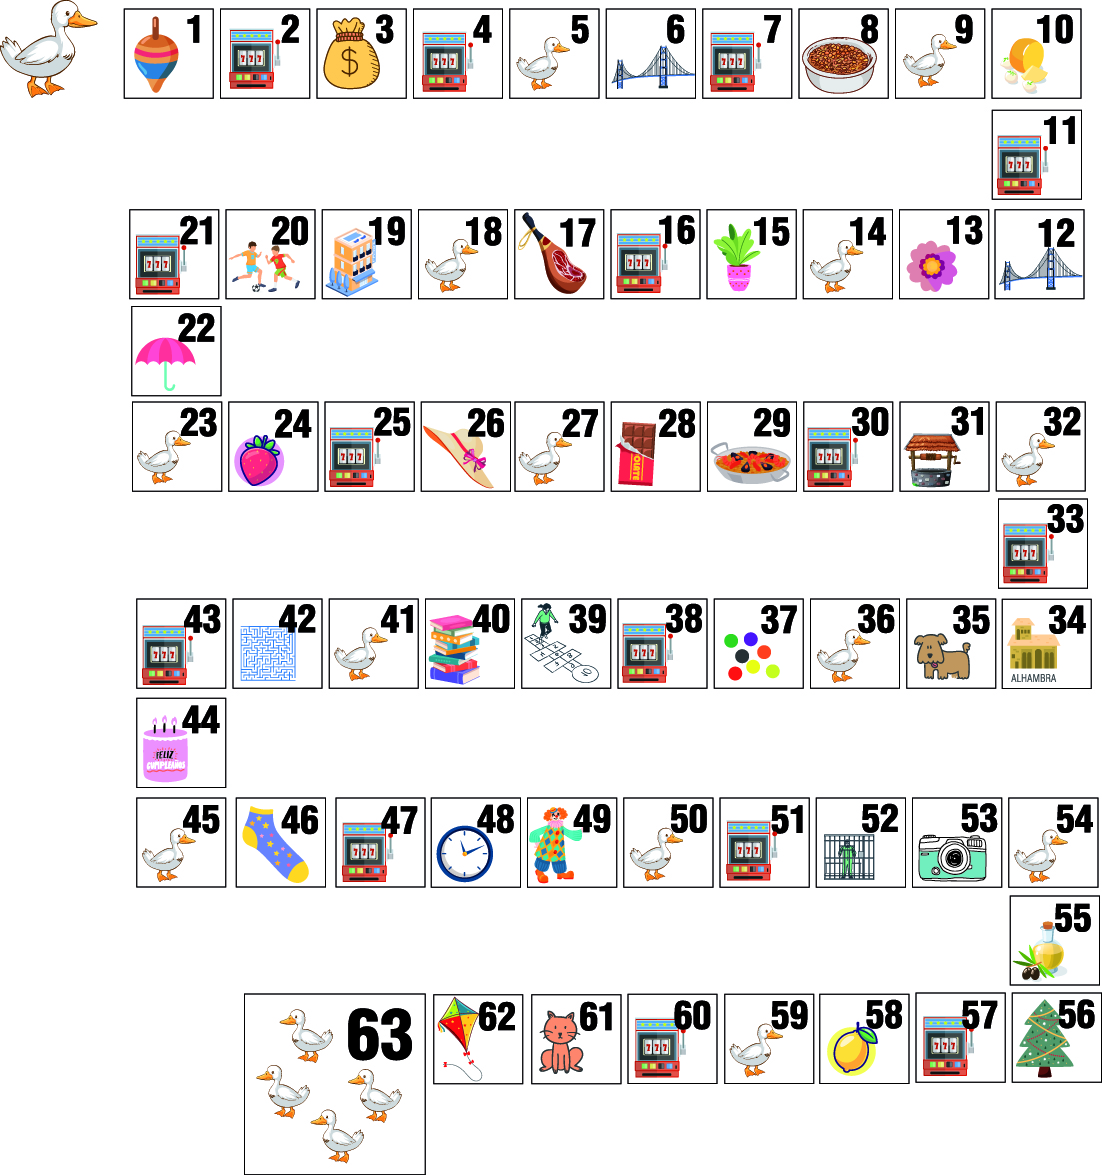
\includegraphics[width=1\textwidth]{imgs/tablero-oca.jpg}
	\caption{Tablero personalizado para la skill del juego de la oca}
	\label{fig:tablero-oca}
\end{figure}
 
Entonces, la distribución de las casillas es la siguiente: 18 especiales tomadas del juego tradicional (oca, puente, laberinto, pozo, cárcel y hotel), 15 de tipo minijuego y 30 normales (no desencadenan ninguna acción especial, salvo la de meta). Por tanto, los porcentajes redondeados de las proporciones de cada una son: 28,57\%, 23,81\% y 47,62\%, respectivamente. 

\subsubsection{Bocetos y mockups}

Para que las personas mayores puedan tener una experiencia de usuario accesible y cómoda, el principio de usabilidad número uno a seguir es mantener un diseño sencillo y minimalista, con elementos claros y bien organizados, contrastes aceptables y tamaños de texto grandes. 

Es lo que se ha tratado de lograr con los siguientes bocetos, que definen la apariencia de la interfaz, habiendo un total de cuatro estados para mantenerlo lo más simple posible. La herramienta empleada es \href{https://www.lucidchart.com/pages/es}{\textit{Lucidchart}}, un software gratuito para el diseño de modelos, diagramas y planificación de procesos y tareas.

En primer lugar se tiene la pantalla de inicio (\autoref{fig:boceto-bienvenida}), cuya mayor parte será ocupada por el logo del juego de la oca, y bajo esta, un texto de bienvenida con un tamaño de fuente considerable. Esta pantalla es la que se mostrará nada más lanzar la skill.

\begin{figure}[H]
    \centering
    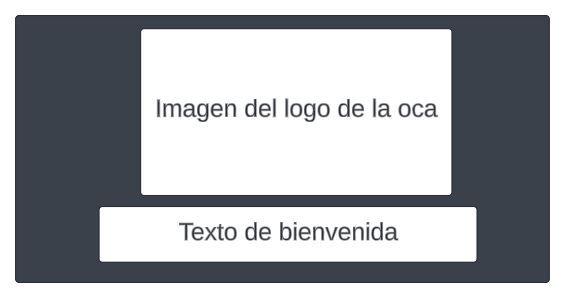
\includegraphics[width=0.5\textwidth]{imgs/boceto-bienvenida.JPG}
    \caption{Boceto de la pantalla de inicio de la skill}
    \label{fig:boceto-bienvenida}
\end{figure}

A continuación, y solo en caso de que se esté creando una partida nueva, se mostrará una pantalla con los nombres de los equipos o participantes, escritos sobre un rectángulo del color que tienen asignado cada uno (\autoref{fig:boceto-fichas}). Esta pantalla servirá como recordatorio o resumen de quienes van a tomar parte en el juego actual.

\begin{figure}[H]
    \centering
    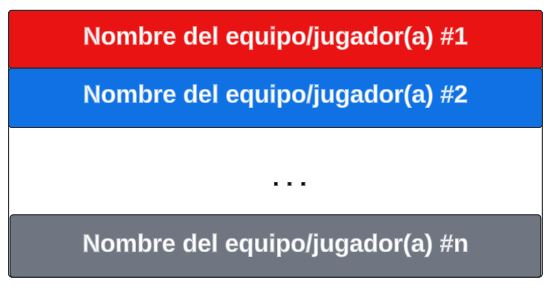
\includegraphics[width=0.5\textwidth]{imgs/boceto-fichas.JPG}
    \caption{Boceto de la pantalla con los participantes}
    \label{fig:boceto-fichas}
\end{figure}

En tercer lugar, debe haber una pantalla que muestre la animación del lanzamiento de dado. Para evitar solapamientos y distracciones, el vídeo ocupará el espacio entero disponible, tal y como aparece en la \autoref{fig:boceto-dado}.

\begin{figure}[H]
	\centering
	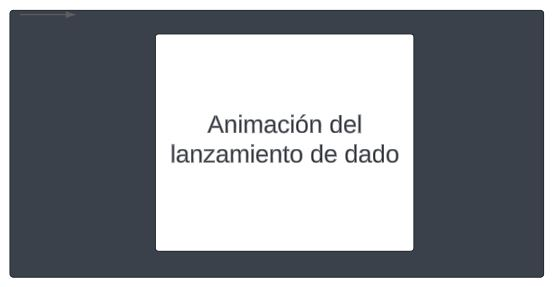
\includegraphics[width=0.5\textwidth]{imgs/boceto-dado.JPG}
	\caption{Boceto de la pantalla de lanzamiento de dado}
	\label{fig:boceto-dado}
\end{figure}

Para finalizar, debe poder visualizarse la posición del equipo o participante actual. Puesto que las dimensiones del dispositivo de Alexa son reducidas, no es conveniente intentar mostrar el tablero entero, por lo que solo se mostrará en la miatd derecha la casilla actual (con su número e imagen representativa), y en la izquierda, las fichas de quienes se encuentran en ella, representadas con un formato idéntico al de la \autoref{fig:boceto-fichas}.

\begin{figure}[H]
	\centering
	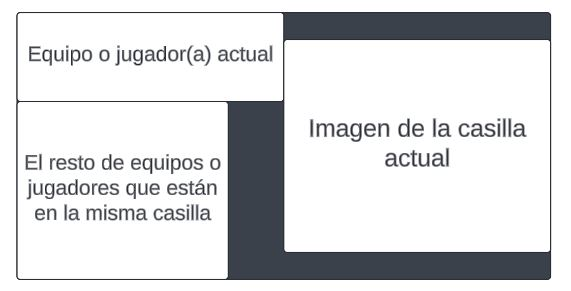
\includegraphics[width=0.5\textwidth]{imgs/boceto-casilla.JPG}
	\caption{Boceto de pantalla con la casilla y participante actual}
	\label{fig:boceto-casilla}
\end{figure}

\newpage

\subsubsection{Diagrama de flujo entre pantallas}

Debido a que solo existen cuatro tipos de pantallas en todo el juego, el diagrama de flujo entre ellas es igual de simple. Pues se pretende que la navegación entre pantallas sea automática e intuitiva, mostrando únicamente los elementos que pueden ayudar a los participantes a visualizar mejor la progresión del juego.

Cabe destacar el papel de la persona terapeuta o guía de la sesión, que será la responsable de configurar la partida antes de empezar a jugar, ya sea introduciendo datos nuevos para crear una desde cero, o cargando la última partida guardada. Por tanto, en la \autoref{fig:diagrama-pantallas} se distinguen tres flujos distintos: 
\begin{itemize}
	\item El primero, indicado en \textit{rojo}, muestra la secuencia desde la pantalla de inicio, pasando por la configuración de participantes, que hay que seguir para poder crear una nueva partida.
	\item El segundo recorrido, representado por el \textit{azul}, omite la fase de configuración y carga los datos de la última partida guardada.
	\item Tanto el camino rojo como el azul desembocan en el \textit{verde}, que representa el flujo de una partida en curso, compuesto por las dos fases principales de un turno: el lanzamiento de dados y el movimiento de la ficha.
\end{itemize}

\begin{figure}[H]
	\centering
	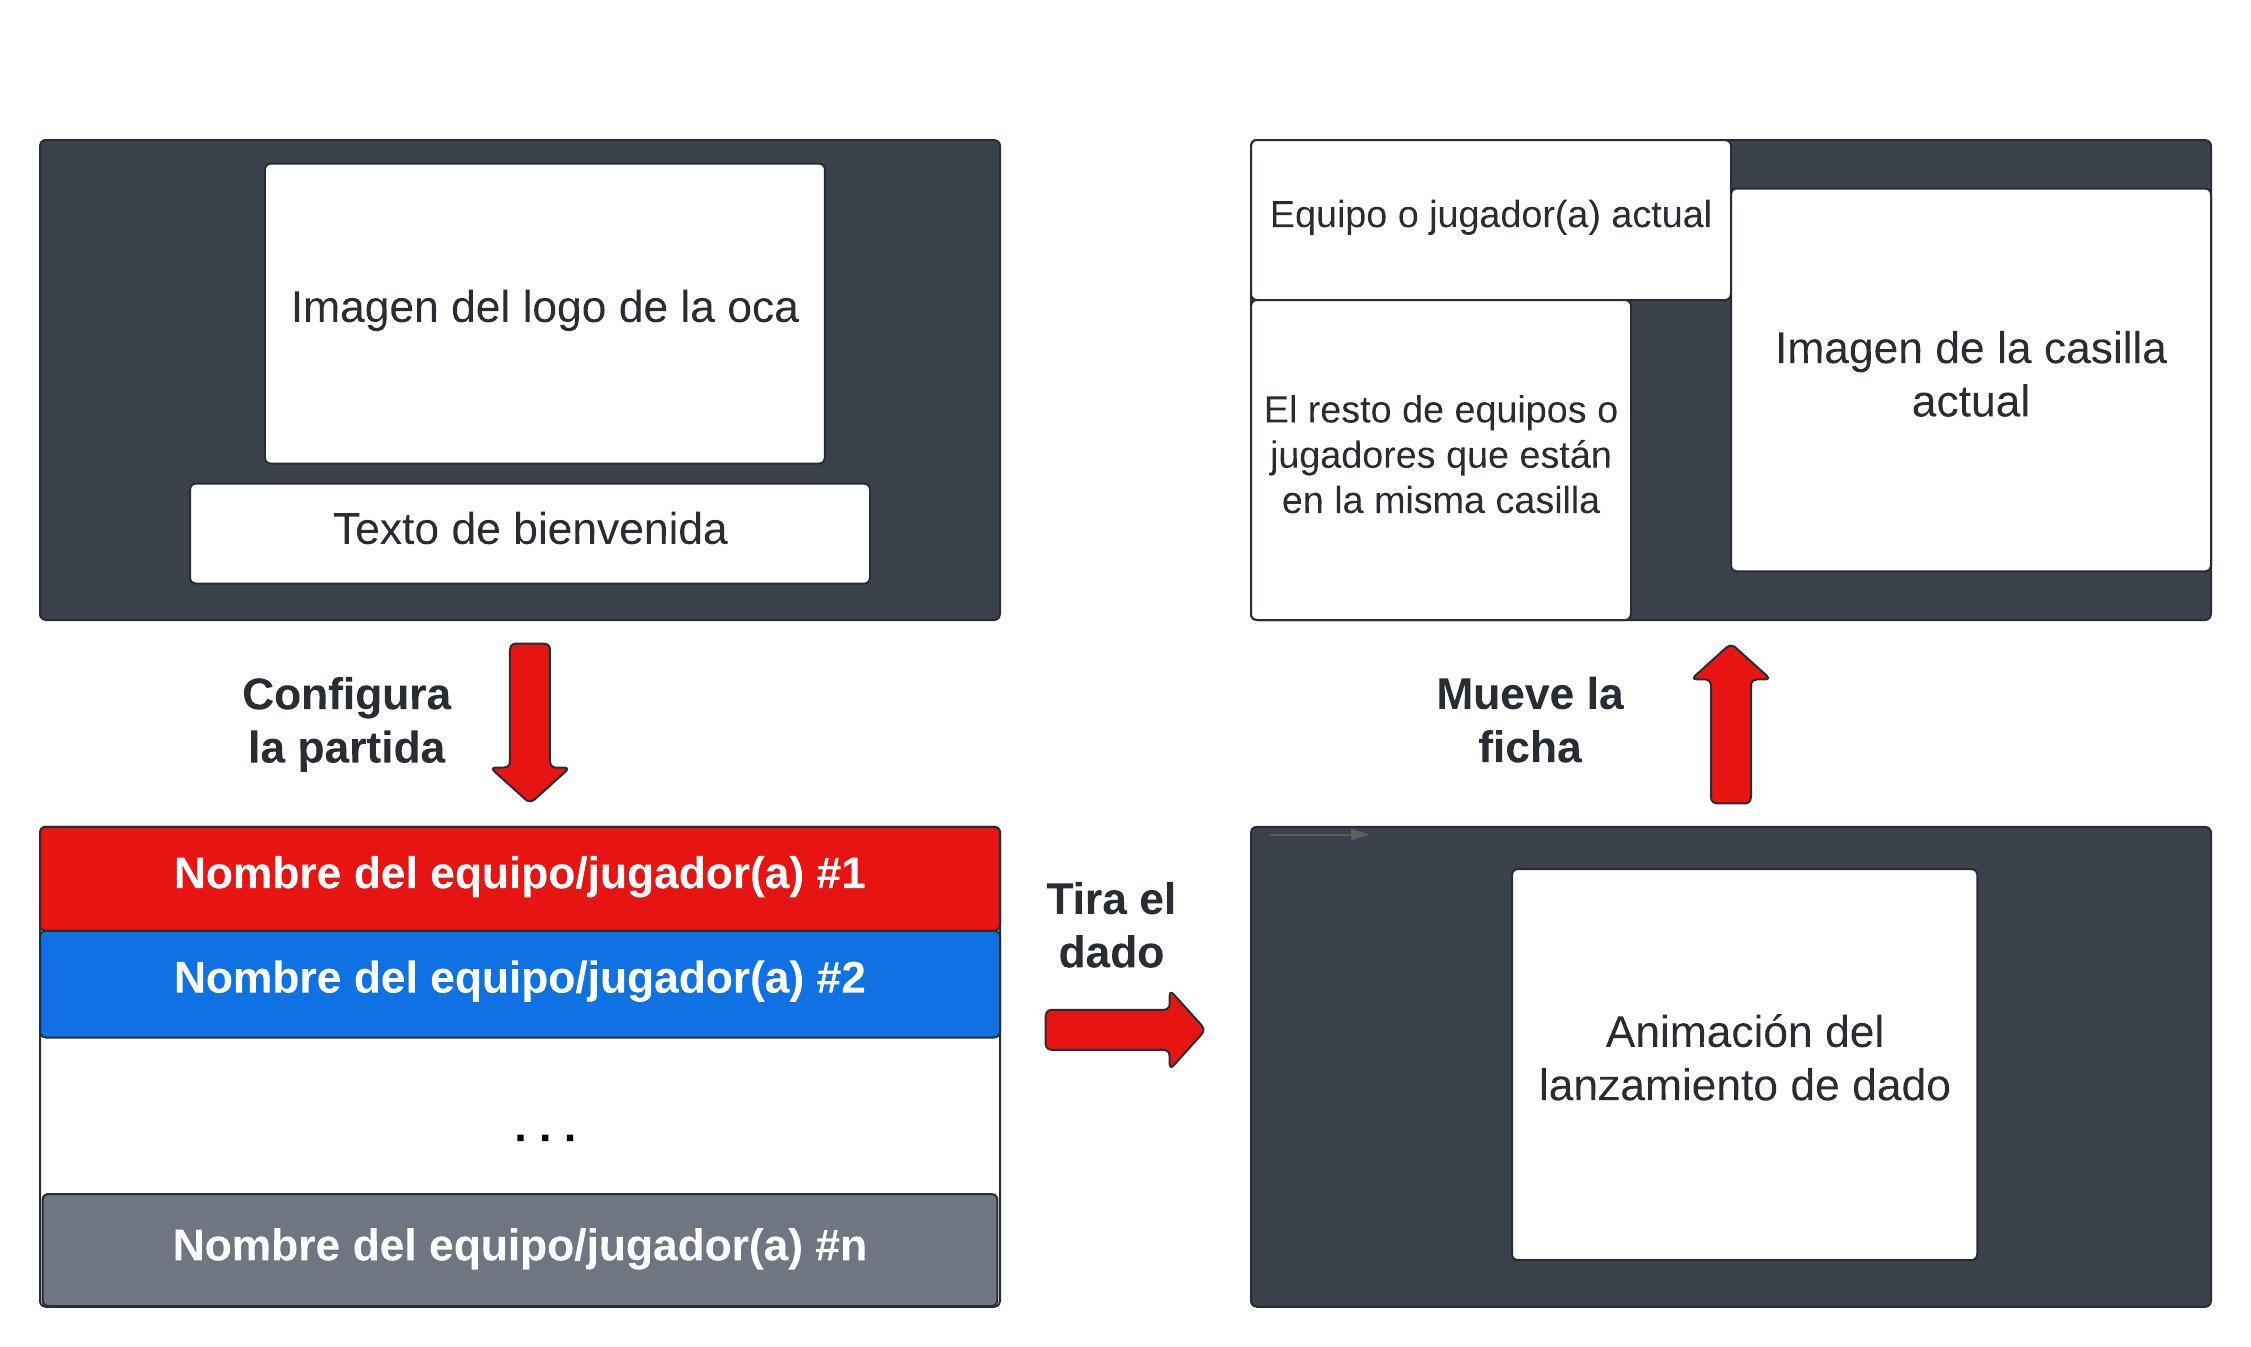
\includegraphics[width=1\textwidth]{imgs/diagrama-pantallas.jpeg}
	\caption{Diagrama de flujo entre pantallas}
	\label{fig:diagrama-pantallas}
\end{figure}

\newpage

\subsubsection{Cuestiones de estética, usabilidad y accesibilidad}

Para el estudio de las variables relevantes a la ergonomía del juego, se ha seguido la metodología utilizada en un juego digital para adultos mayores llamado \textit{Solitaire Quiz}. Este está inspirado en el \textit{Solitario}, un juego de cartas tradicional, y a diferencia del original, incluye contenidos didácticos en forma de pequeños cuestionarios \parencite{diseño2017}.

\begin{table}[H]
	\centering
	\begin{tabular}{|c|p{6cm}|}
		\hline
		\rowcolor{lightgray}
		\textbf{Categoría} & \textbf{Variables}\\
		\hline
		\multirow{3}{*}{Diseño del juego} & - Desafío \\
		& - Contenido del aprendizaje \\
		& - Retroalimentación \\
		\hline
		\multirow{4}{*}{Usabilidad} & - Ambiente externo al juego \\
		& - Ambiente interno al juego \\
		& - Elementos visuales \\
		& - Dispositivos \\
		\hline
		\multirow{3}{*}{Legibilidad} & - Texto \\
		& - Imágenes \\
		& - Audio \\
		\hline
	\end{tabular}
	\caption{Dimensiones y variables de la ergonomía de la app}
	\label{tab:usabilidad}
\end{table}

Partiendo del Cuadro \ref{tab:usabilidad}, se han considerado los siguientes aspectos de diseño:

\begin{itemize}
	\item \textbf{Desafío y contenidos de aprendizaje}: hace referencia al nivel de dificultad, por ejemplo, en el contexto de los minijuegos integrados en el juego de la oca. Se ha pensado a la hora de preparar las preguntas en el público objetivo al que van a ir dirigidas, es decir, personas mayores con un nivel educativo entre medio y bajo. De esta manera, las preguntas son sencillas y directas, sin dobles sentidos.
	\item \textbf{Retroalimentación}: se ha tenido en cuenta experiencias recogidas en estudios publicados en el área de la Gerontología por profesionales de la psicología y la salud a favor de la integración social de los mayores. En este sentido, los minijuegos integrados ya se habían validado por una psicóloga en residencias para asegurar su viabilidad.
	\item \textbf{Ambiente externo al juego}: es el entorno previo a cada partida. El proceso de configuración debe estar guiado y ser intuitivo. Se debe acordar cuántas personas van a jugar, el orden, la manera de intervenir y se recomienda hacer pruebas para interactuar con Alexa de manera práctica.
	\item \textbf{Ambiente interno al juego}: durante la partida es importante respetar los turnos de los jugadores y jugadoras para evitar errores, pero la skill está diseñada para ser flexible a la hora de manejar los errores que puedan surgir, o bien porque algún participante ha perdido el hilo de la partida o se ha equivocado de frase.
	\item \textbf{Elementos visuales}: los escogidos para el juego, además de ser atractivos a la vista se han escogido para que cuando se muestan en la pantalla de Alexa ayuden a entender mejor el estado actual y no distraigan, por ello debe ser un diseño simple y minimalista.
	\item \textbf{Dispositivo}: se requiere un solo dispositivo Alexa con pantalla para poder jugar. Al grupo de jugadores y jugadoras se les habrá de explicar cómo es el desarrollo, ya que que toda la interacción es por voz. En cualquier caso y si hay dudas se les proporcionará un manual de uso, y existen opciones de pedir ayuda.  
	\item \textbf{Texto}: para que no presenten a las personas jugadoras problemas de legibilidad con la pantalla se ha tenido en cuenta esta posibilidad y se han incluido tipos de letra grandes y una buena definición de colores
	\item \textbf{Imágenes}: son de unas dimensiones considerables y muy representativas. Todas las casillas se representan por un solo elemento para mayor simplicidad y evitar confusión en el desarrollo del juego. 
	\item \textbf{Audio}: es otro de los elementos imprescindibles del juego, al ser toda la interacción por voz no hay efectos de sonido que puedan distraer u obstruir el flujo de conversación.
\end{itemize}


